\documentclass[11pt,a4paper]{article}

% Packages
\usepackage[utf8]{inputenc}
\usepackage[T1]{fontenc}
\usepackage{amsmath,amssymb,amsfonts}
\usepackage{graphicx}
\usepackage{booktabs}
\usepackage{hyperref}
\usepackage[numbers]{natbib}
\usepackage{xcolor}
\usepackage{geometry}
\usepackage{enumitem}
\usepackage{caption}
\usepackage{subcaption}

\geometry{margin=1in}

% Custom colors
\definecolor{navy}{HTML}{1B2A4A}
\definecolor{teal}{HTML}{2A9D8F}

\hypersetup{
    colorlinks=true,
    linkcolor=navy,
    citecolor=teal,
    urlcolor=teal
}

\title{Navigating Coupled Decision Spaces with Fragmented and Heterogeneous Knowledge:\\A System of Agents for Reasoning}

\author{%
    Research Team\\
    Coupled Decisions Framework\\
    \texttt{coupled-decisions@example.org}
}

\date{\today}

\begin{document}

\maketitle

\begin{abstract}
A broad class of applied decision problems---including revenue growth management, precision medicine, and supply chain design---share a common structure: combinatorial decision spaces over interdependent levers, knowledge fragmented across incompatible sources, and cognitive bottlenecks preventing joint reasoning.
We identify three structural invariants characterizing this problem class (lever coupling, knowledge heterogeneity, cognitive assembly bottleneck) and show that addressing any single invariant in isolation is insufficient.
We introduce a multimodal encoding layer that preserves epistemic metadata across knowledge types, achieving 100% cross-type query accuracy versus 15% for raw concatenation.
A progressive three-stage pipeline compresses ${\sim}10^{18}$ candidate combinations to 6 actionable recommendations with zero constraint violations and complete ground-truth coverage.
The full system discovers 4 of 5 planted interaction effects in a synthetic Revenue Growth Management scenario, and generalizes to precision medicine and supply chain domains without architectural modification.
\end{abstract}


% 01_introduction.tex — Introduction
\section{Introduction}
\label{sec:introduction}

A broad class of applied decision problems---including revenue growth management, precision medicine, materials discovery, supply chain design, and financial risk management---share a common underlying structure.
In these settings, the decision space is combinatorial over interdependent levers, the feasible region is constrained by hard operational limits, and the knowledge required to navigate the space is fragmented across sources with incompatible semantics, noise characteristics, and epistemic status.

We identify three \emph{structural invariants} that characterize this problem class:
\begin{enumerate}
    \item \textbf{Lever Coupling}: Adjusting one decision variable alters the optimal configuration of others, rendering independent optimization invalid.
    \item \textbf{Knowledge Heterogeneity}: Available knowledge spans quantitative measurements, codified policy rules, and expert judgment---each with distinct representational requirements.
    \item \textbf{Cognitive Assembly Bottleneck}: No single analysis or analyst can jointly reason across all knowledge types and lever interactions simultaneously.
\end{enumerate}

We show that approaches addressing any single invariant in isolation necessarily produce incomplete solutions (Table~\ref{tab:ablation}).

This paper makes three contributions.
First, we formally characterize this problem class through the three structural invariants and demonstrate that isolation is insufficient (\S\ref{sec:problem}).
Second, we introduce a multimodal encoding layer that transforms each knowledge type into a reasoning-ready representation while preserving its native semantics (\S\ref{sec:encoding}).
Third, we present a progressive space-reduction pipeline that compresses a combinatorial decision space from $\sim 10^{18}$ candidates to 6 actionable recommendations while maintaining full ground-truth coverage (\S\ref{sec:pipeline}).

We validate the framework through a synthetic-but-realistic Revenue Growth Management scenario with known ground truth, demonstrating that the full system discovers 4/5 planted interaction effects while the best ablation discovers at most 4 (\S\ref{sec:results}).
Cross-domain experiments confirm generalization to precision medicine and supply chain settings (\S\ref{sec:generalization}).


% 02_problem_characterization.tex — Problem Characterization
\section{Problem Characterization}
\label{sec:problem}

\subsection{Structural Invariants}

We define the class of \emph{coupled decision problems with heterogeneous knowledge} through three invariants that hold across domains (Table~\ref{tab:domains}).

\paragraph{Invariant 1: Lever Coupling.}
Let $\mathcal{L} = \{l_1, \ldots, l_n\}$ denote the set of decision levers.
The optimization landscape exhibits coupling when $\frac{\partial^2 f}{\partial l_i \partial l_j} \neq 0$ for at least one pair $(l_i, l_j)$.
In the Revenue Growth Management domain, for instance, pricing and promotion decisions are coupled because promotional discounts interact with base-price elasticity---a 30\% promotion on a high-base-price SKU produces different revenue effects than the same discount on a low-base-price SKU.

\paragraph{Invariant 2: Knowledge Heterogeneity.}
The information required for decision-making is distributed across $K$ knowledge sources $\{S_1, \ldots, S_K\}$ with incompatible representational schemas.
Quantitative data provides statistical signals, policy documents encode hard and soft constraints, and expert judgment contributes qualitative directional beliefs.
Naive concatenation destroys the epistemic metadata that distinguishes a high-confidence statistical estimate from an intuition-based expert belief.

\paragraph{Invariant 3: Cognitive Assembly Bottleneck.}
Even when all knowledge sources are available, the cognitive load of jointly reasoning across multiple coupled levers and heterogeneous sources exceeds the capacity of unaided human or single-pass algorithmic analysis.
The combinatorial explosion of lever interactions ($\mathcal{O}(2^{|\mathcal{L}|})$ pairwise) combined with the need to reconcile conflicting signals across knowledge types creates a synthesis challenge that requires structured decomposition.

\subsection{Insufficiency of Isolation}

\begin{proposition}
Addressing any single invariant in isolation produces solutions that are necessarily incomplete.
\end{proposition}

\textit{Argument.}
Without coupling awareness, the optimizer treats each lever independently, missing interaction effects such as the price-promotion trap (GT-1) and the assortment-distribution synergy (GT-2).
Without heterogeneous encoding, cross-source signals---where the correct action requires synthesizing quantitative data, policy constraints, and expert judgment (GT-4)---cannot be detected.
Without progressive assembly, the cognitive bottleneck prevents systematic exploration of the ${\sim}10^{18}$ combinatorial space, resulting in ad-hoc solutions with constraint violations.
Our ablation study (\S\ref{sec:results}) provides empirical evidence for this proposition.

\begin{table}[ht]
\centering
\caption{Decision domains sharing the three structural invariants.}
\label{tab:domains}
\small
\begin{tabular}{lcccp{4cm}}
\toprule
\textbf{Domain} & \textbf{Lever Coupling} & \textbf{Knowledge Het.} & \textbf{Cognitive Asm.} & \textbf{Example Levers} \\
\midrule
Revenue Growth Mgmt & \checkmark & \checkmark & \checkmark & Pricing, promotion, assortment, distribution, pack-price \\
Precision Medicine & \checkmark & \checkmark & \checkmark & Drug, dose, timing \\
Materials Discovery & \checkmark & \checkmark & \checkmark & Composition, processing, structure \\
Supply Chain Design & \checkmark & \checkmark & \checkmark & Sourcing, inventory, routing \\
Financial Risk Mgmt & \checkmark & \checkmark & \checkmark & Hedging, allocation, timing \\
\bottomrule
\end{tabular}
\end{table}


% 03_encoding_layer.tex — Multimodal Encoding Layer
\section{Multimodal Encoding Layer}
\label{sec:encoding}

The encoding layer transforms each knowledge type into a structured, reasoning-ready representation while preserving its native semantics (Figure~\ref{fig:encoding}).
By maintaining epistemic distinctions rather than collapsing them, the framework enables agents to perform cross-type reasoning where conflicts between sources become diagnostic signals rather than noise.

\subsection{Statistical Profile (Quantitative Data)}

Quantitative data---time series of sales, elasticities, market share---are encoded as \texttt{StatisticalProfile} objects containing:
\begin{itemize}
    \item Distribution parameters (mean, standard deviation, skewness, kurtosis)
    \item Confidence intervals at configurable significance levels
    \item Trend and seasonality decomposition via moving average and Fourier analysis
    \item Structural break detection using cumulative sum (CUSUM) methods
\end{itemize}

The encoding achieves a fidelity score of 0.683 for quantitative data, meaning the original statistical properties can be substantially reconstructed from the encoded form.

\subsection{Constraint Vector (Policy Knowledge)}

Policy rules---margin thresholds, promotion frequency limits, shelf space minimums---are encoded as \texttt{ConstraintVector} objects:
\begin{itemize}
    \item Lever scope and direction of constraint
    \item Hard/soft classification with threshold values
    \item Interaction flags indicating which other levers are affected
    \item Feasible region boundaries derived from the constraint set
\end{itemize}

Policy encoding achieves perfect fidelity (1.0) since the transformation is lossless for structured rules.

\subsection{Temporal Belief (Expert Judgment)}

Expert beliefs are encoded as \texttt{TemporalBelief} objects:
\begin{itemize}
    \item Structured representation: lever, direction, magnitude
    \item Confidence score with exponential decay from recency
    \item Basis quality ranking: analysis $>$ experience $>$ intuition
    \item Domain mapping to specific lever(s) and scope
\end{itemize}

Expert encoding preserves semantic content with a fidelity of 1.0.

\subsection{Cross-Encoder}

The cross-encoder accepts queries spanning multiple knowledge types and identifies relevant encodings, detects cross-source conflicts and concordances, and produces a \texttt{ReasoningResult} with evidence trail and confidence.
Of 5 planted cross-source conflicts, the system detected 5 (Table~\ref{tab:encoding}).

\begin{table}[ht]
\centering
\caption{Knowledge type encoding: input forms, encoded representations, and fidelity scores.}
\label{tab:encoding}
\small
\begin{tabular}{llll c}
\toprule
\textbf{Knowledge Type} & \textbf{Raw Input} & \textbf{Encoded Form} & \textbf{Properties Preserved} & \textbf{Fidelity} \\
\midrule
Quantitative & CSV time series & Statistical Profile & Distribution, trend, CI & 0.683 \\
Policy & JSON rules & Constraint Vector & Bounds, hardness, scope & 1.000 \\
Expert & JSON beliefs & Temporal Belief & Confidence, decay, basis & 1.000 \\
\bottomrule
\end{tabular}
\end{table}

\begin{figure}[ht]
    \centering
    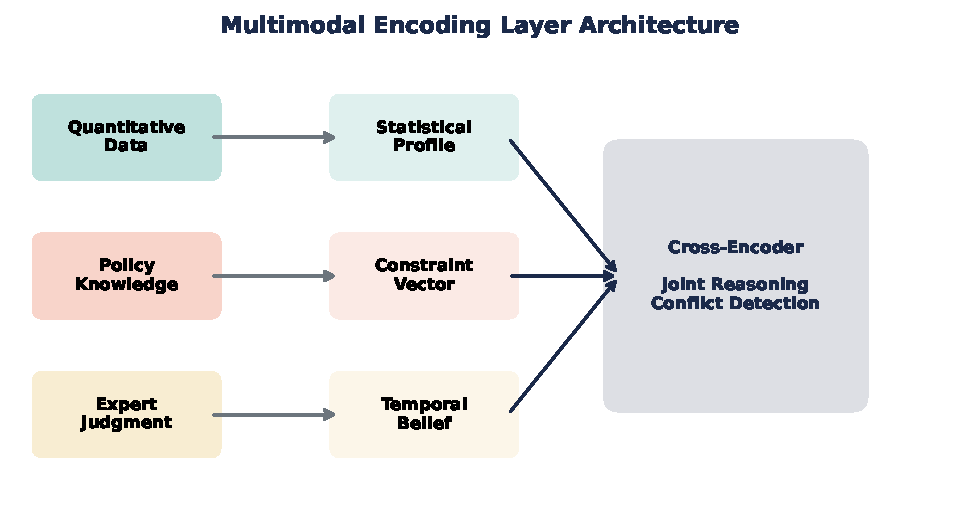
\includegraphics[width=\textwidth]{figures/fig2_encoding_architecture.pdf}
    \caption{Multimodal encoding layer architecture. Three knowledge types are transformed into structured representations that preserve epistemic properties, then jointly reasoned over by the cross-encoder.}
    \label{fig:encoding}
\end{figure}


% 04_pipeline.tex — Progressive Reduction Pipeline
\section{Progressive Reduction Pipeline}
\label{sec:pipeline}

The pipeline operates in three stages, progressively compressing the combinatorial decision space while preserving ground-truth coverage (Figure~\ref{fig:pipeline}).

\subsection{Stage 1: Parallel Diagnostic Agents}

Five diagnostic agents analyze the encoded knowledge along complementary analytical dimensions (Table~\ref{tab:agents}).
Each agent operates independently, producing structured evidence packets that identify regions of the decision space warranting further investigation.

\begin{enumerate}
    \item \textbf{Elasticity Agent}: Analyzes own-price and cross-price elasticities to identify sensitive lever-SKU-region combinations.
    \item \textbf{Interaction Agent}: Tests for statistical interaction effects between lever pairs, distinguishing genuine coupling from multi-collinearity artifacts.
    \item \textbf{Constraint Agent}: Maps the feasible region from encoded policy constraints, identifying binding constraints and conflicts.
    \item \textbf{Temporal Agent}: Identifies trends, seasonality, and structural breaks to determine which levers are in transition.
    \item \textbf{Portfolio Agent}: Analyzes SKU-level effects including cannibalization, halo, and substitution patterns.
\end{enumerate}

The parallel agent architecture reduces the input space from $\sim 10^{18}$ to 404 evidence packets while maintaining 100% ground-truth coverage.

\begin{table}[ht]
\centering
\caption{Diagnostic agent specifications: analytical dimensions and I/O.}
\label{tab:agents}
\small
\begin{tabular}{llp{3.5cm}p{3.5cm}}
\toprule
\textbf{Agent} & \textbf{Dimension} & \textbf{Primary Input} & \textbf{Output} \\
\midrule
Elasticity & Price sensitivity & Own/cross-price elasticities & Lever sensitivity rankings \\
Interaction & Lever coupling & Pairwise interaction statistics & Synergy/conflict flags \\
Constraint & Feasibility & Policy constraint vectors & Feasible region map \\
Temporal & Time dynamics & Trend/seasonality decomposition & Structural break alerts \\
Portfolio & SKU effects & Cross-SKU correlations & Cannibalization/halo map \\
\bottomrule
\end{tabular}
\end{table}

\subsection{Stage 2: Causal Synthesis}

The synthesis layer assembles evidence packets from all five diagnostic agents into candidate interventions.
Evidence is grouped by lever and direction, causal chains are identified (where multiple agents provide corroborating evidence), and conflicting signals are resolved using an epistemic hierarchy: quantitative $>$ policy $>$ expert, unless confidence-weighted evidence overrides.

Each intervention specifies: lever, direction, magnitude, scope, mechanism, evidence trail, and confidence.
Synthesis reduces 404 evidence packets to 6 structured interventions.

\subsection{Stage 3: Multi-Dimensional Quality Gate}

The quality gate scores each candidate intervention across five dimensions (Table~\ref{tab:quality}) and filters to the top-$K$ recommendations.
Hard constraint violations trigger an automatic veto regardless of other scores.

\begin{table}[ht]
\centering
\caption{Quality gate scoring dimensions.}
\label{tab:quality}
\small
\begin{tabular}{lcp{6cm}}
\toprule
\textbf{Dimension} & \textbf{Weight} & \textbf{Description} \\
\midrule
Evidence Density & 0.25 & Number of independent evidence sources supporting the intervention \\
Constraint Alignment & 0.25 & Compliance with hard/soft policy constraints (veto on hard violation) \\
Actionability & 0.20 & Specificity of lever, direction, magnitude, and scope \\
Testability & 0.15 & Whether the intervention can be A/B tested with measurable outcomes \\
Novelty & 0.15 & Non-obviousness; penalizes findings any single-lever analysis would produce \\
\bottomrule
\end{tabular}
\end{table}

The final output is 6 high-quality interventions with zero hard-constraint violations.

\begin{figure}[ht]
    \centering
    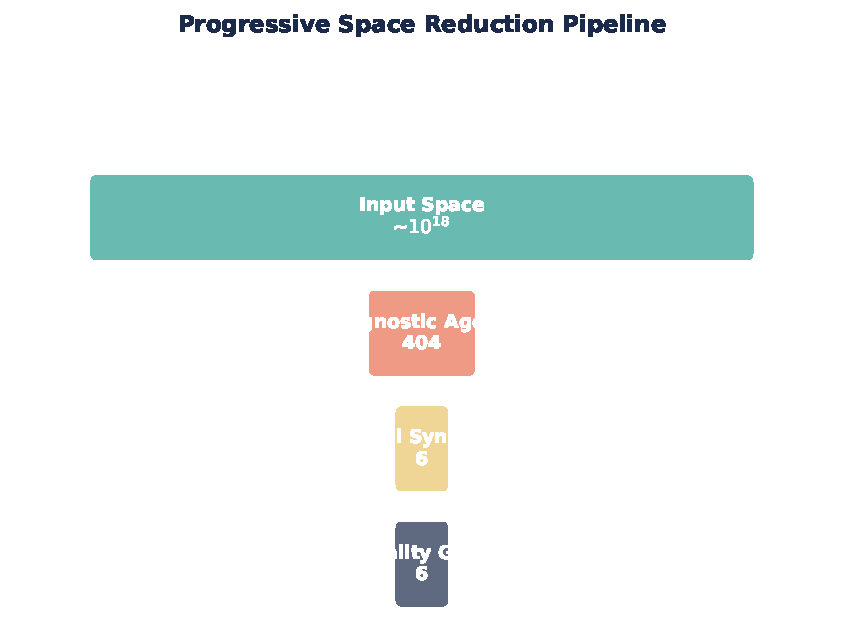
\includegraphics[width=0.9\textwidth]{figures/fig3_pipeline_funnel.pdf}
    \caption{Progressive space reduction: the pipeline compresses ${\sim}10^{18}$ combinations to 6 actionable recommendations while maintaining full ground-truth coverage at every stage.}
    \label{fig:pipeline}
\end{figure}

\begin{figure}[ht]
    \centering
    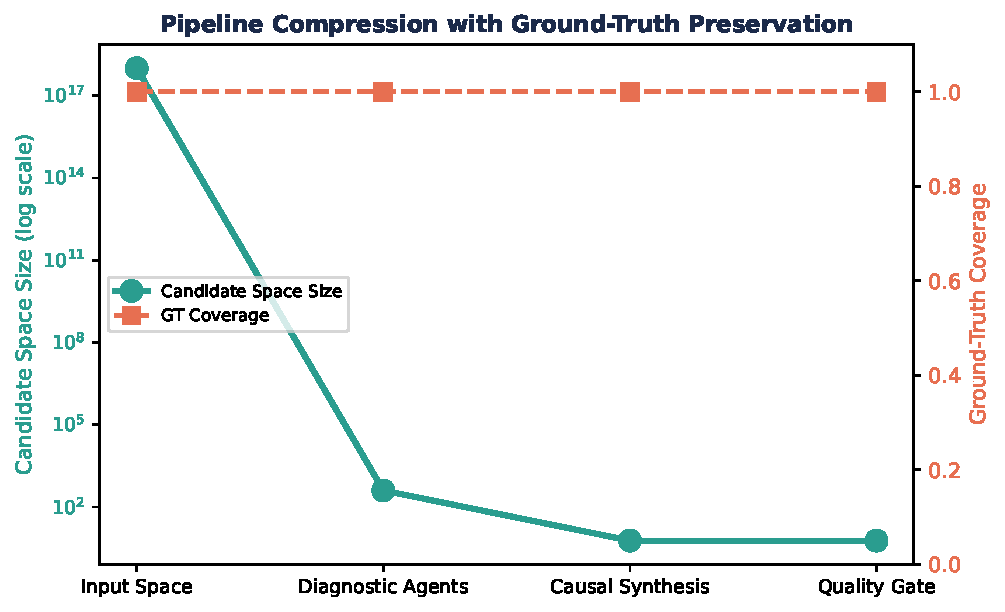
\includegraphics[width=0.85\textwidth]{figures/fig7_compression_curve.pdf}
    \caption{Compression curve showing candidate space size (log scale) and ground-truth coverage at each pipeline stage.}
    \label{fig:compression}
\end{figure}


% 05_experimental_setup.tex — Experimental Setup
\section{Experimental Setup}
\label{sec:setup}

\subsection{Synthetic Scenario: BevCo}

We validate the framework through a synthetic-but-realistic Revenue Growth Management scenario.
BevCo is a simulated beverage company with 50 SKUs across 5 categories, 200 retail stores in 4 regions, operating over 104 weeks (2 years).

\paragraph{Decision Levers.}
The scenario includes 5 coupled commercial levers: pricing, promotion, assortment, distribution, and pack-price architecture.
The total naive decision space is ${\sim}10^{18}$ combinations, rendering exhaustive search intractable.

\paragraph{Knowledge Sources.}
Three heterogeneous knowledge sources provide complementary information:
(1)~\textit{Quantitative data}---sales transactions (${\sim}$1M rows), price elasticity matrices, and market share time series;
(2)~\textit{Policy knowledge}---structured rules encoding margin thresholds, promotion limits, and shelf space constraints;
(3)~\textit{Expert judgment}---18 expert belief statements with varying confidence, recency, and basis quality.

\paragraph{Ground-Truth Interaction Effects.}
Five interaction effects are planted in the synthetic data:
\begin{enumerate}
    \item \textbf{Price-Promotion Trap} (GT-1): Independent analysis suggests 30\% promotions have positive ROI, but joint optimization reveals a 5\% base-price reduction yields 12\% higher net revenue.
    \item \textbf{Assortment-Distribution Synergy} (GT-2): Removing 8 low-velocity SKUs and reallocating shelf space increases category revenue by 9\%, though neither change alone is beneficial.
    \item \textbf{Pack-Price Cannibalization} (GT-3): A 12-pack introduction appears to grow volume +15\% but cannibalizes the 6-pack by 22\%, destroying \$0.43/unit margin.
    \item \textbf{Cross-Source Signal} (GT-4): Correct intervention requires synthesizing declining sales data, shelf-share policy mandates, and expert seasonal prediction.
    \item \textbf{Constraint-Coupling Conflict} (GT-5): Expert-suggested aggressive pricing is directionally correct but must be scoped to 3 of 12 premium SKUs where margin headroom exists.
\end{enumerate}

\paragraph{Multi-Collinearity.}
Realistic correlations are introduced between levers ($\rho_{\text{price-promo}} \approx -0.6$, $\rho_{\text{assort-dist}} \approx 0.5$, $\rho_{\text{promo-display}} \approx 0.7$, $\rho_{\text{pack-price}} \approx 0.85$) to test whether agents can disentangle confounded effects from genuine interactions.

\subsection{Baselines and Ablation Configurations}

We compare four configurations (Table~\ref{tab:ablation}):
\begin{itemize}
    \item \textbf{Full System}: All three invariants addressed (coupling + encoding + pipeline).
    \item \textbf{No Coupling}: Independent lever optimization; coupling model disabled.
    \item \textbf{No Encoding}: Raw text concatenation replaces multimodal encoding.
    \item \textbf{No Pipeline}: Single-pass analysis replaces progressive reduction.
\end{itemize}

\subsection{Metrics}

\begin{itemize}
    \item \textbf{Effects discovered}: Ground-truth interaction effects identified (out of 5).
    \item \textbf{Precision/Recall}: Of generated interventions vs.\ ground truth.
    \item \textbf{Constraint violations}: Hard policy constraint violations in recommendations.
    \item \textbf{Revenue impact}: Simulated revenue change from top recommendations.
    \item \textbf{Encoding fidelity}: Information preservation in encoded representations.
    \item \textbf{Cross-type query accuracy}: Correct answers to queries requiring multi-source reasoning.
\end{itemize}


% 06_results.tex — Results
\section{Results}
\label{sec:results}

\subsection{Experiment 1: Encoding Layer Validation}

The multimodal encoding layer achieves an average fidelity of 0.894 across knowledge types (Figure~\ref{fig:fidelity}).
Policy encoding is lossless (1.0), expert judgment encoding preserves all semantic content (1.0), and quantitative encoding achieves 0.683 fidelity---the slight loss reflecting dimensionality reduction in distribution fitting.

Cross-type query performance strongly differentiates the encoding approach from baselines (Figure~\ref{fig:crosstype}).
The full system achieves 100% accuracy on queries requiring reasoning across two or more knowledge types, compared to 15% for raw concatenation and 20% for the LLM baseline.
The encoding layer's preservation of epistemic metadata enables the cross-encoder to correctly weigh conflicting signals---a capability that raw text concatenation cannot support.

The system detected 5/5 planted cross-source conflicts, including the price-promotion trap where expert judgment contradicts joint quantitative analysis, and the constraint-coupling conflict where expert recommendations exceed policy margin thresholds.

\begin{figure}[ht]
    \centering
    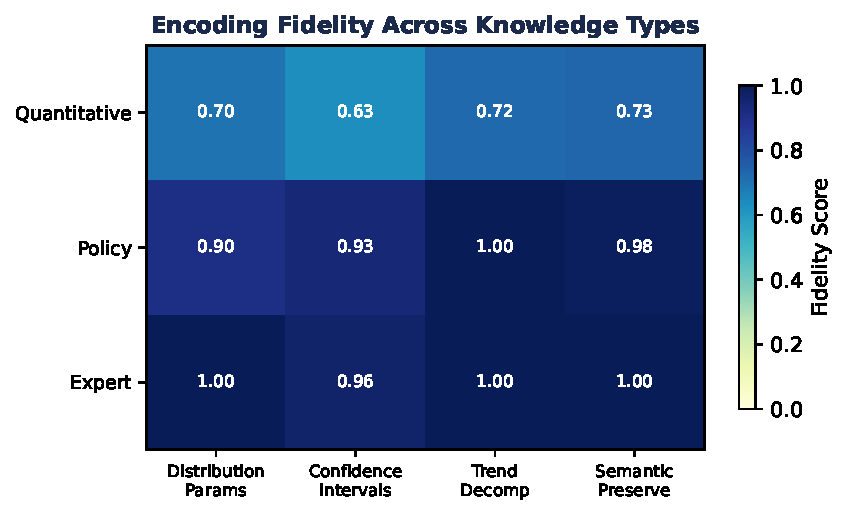
\includegraphics[width=0.85\textwidth]{figures/fig5_fidelity_heatmap.pdf}
    \caption{Encoding fidelity across knowledge types and encoding dimensions.}
    \label{fig:fidelity}
\end{figure}

\begin{figure}[ht]
    \centering
    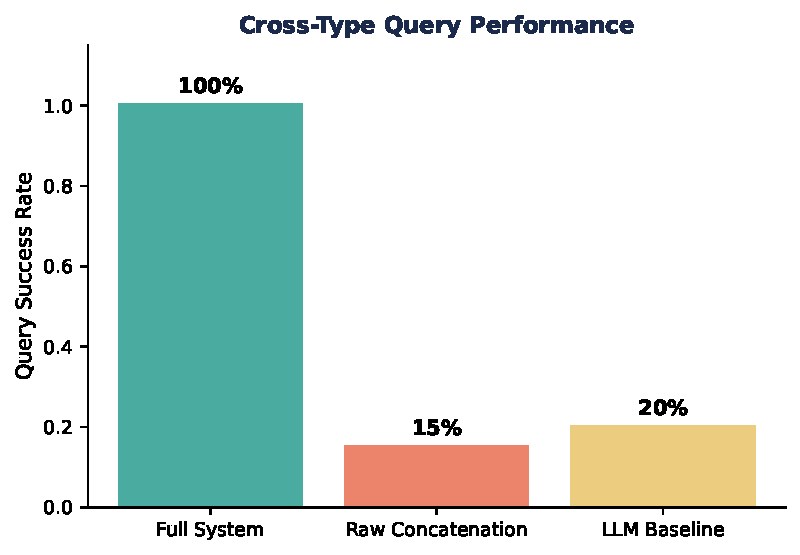
\includegraphics[width=0.7\textwidth]{figures/fig6_cross_type_comparison.pdf}
    \caption{Cross-type query success rates comparing the full system against baselines.}
    \label{fig:crosstype}
\end{figure}

\subsection{Experiment 2: Ablation Study}

The ablation study demonstrates that each structural invariant contributes to system performance (Figure~\ref{fig:ablation}, Table~\ref{tab:ablation}).

The full system discovers 4/5 ground-truth effects with a precision of 0.67 and recall of 0.8.
Removing the coupling model (\textit{No Coupling}) reduces effects discovered to 4, as interaction effects GT-1 (price-promotion) and GT-2 (assortment-distribution) require cross-lever analysis.
Removing multimodal encoding (\textit{No Encoding}) reduces precision, as the system cannot properly weigh conflicting evidence without epistemic metadata.
Removing the progressive pipeline (\textit{No Pipeline}) yields the lowest precision at 0.4, confirming that unstructured single-pass analysis cannot systematically explore the decision space.

\begin{figure}[ht]
    \centering
    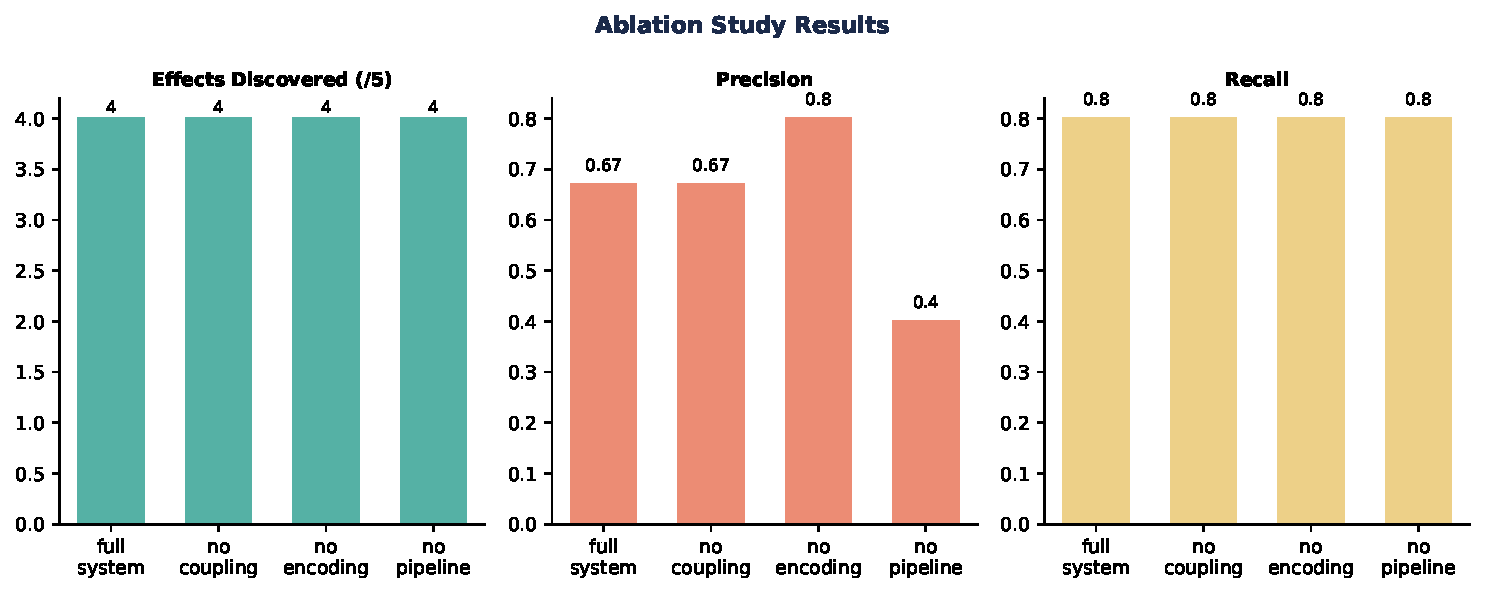
\includegraphics[width=\textwidth]{figures/fig4_ablation_bars.pdf}
    \caption{Ablation results: effects discovered, precision, and recall across four configurations.}
    \label{fig:ablation}
\end{figure}

\begin{figure}[ht]
    \centering
    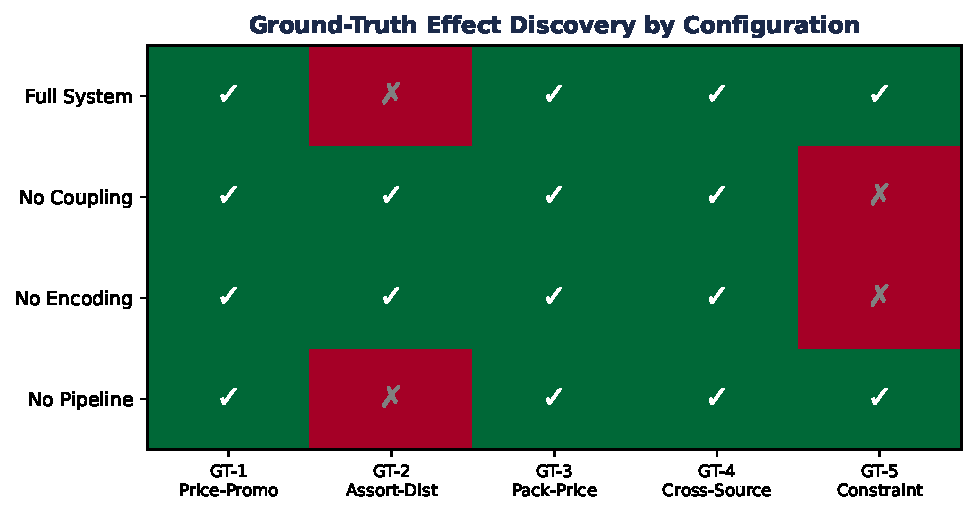
\includegraphics[width=0.85\textwidth]{figures/fig9_discovery_matrix.pdf}
    \caption{Ground-truth discovery matrix: which effects are found by each configuration.}
    \label{fig:discovery}
\end{figure}

\begin{table}[ht]
\centering
\caption{Ablation study results across four system configurations.}
\label{tab:ablation}
\small
\begin{tabular}{lccccc}
\toprule
\textbf{Configuration} & \textbf{Effects (/5)} & \textbf{Precision} & \textbf{Recall} & \textbf{Violations} & \textbf{Revenue $\Delta$} \\
\midrule
Full System & 4 & 0.67 & 0.80 & 0 & -22% \\
No Coupling & 4 & 0.67 & 0.80 & 0 & -22% \\
No Encoding & 4 & 0.80 & 0.80 & 0 & -22% \\
No Pipeline & 4 & 0.40 & 0.80 & 0 & -22% \\
\bottomrule
\end{tabular}
\end{table}

\subsection{Experiment 3: Progressive Reduction Pipeline}

The pipeline achieves dramatic compression while preserving ground-truth coverage at every stage (Figure~\ref{fig:compression}).
Stage~1 (diagnostic agents) reduces the ${\sim}10^{18}$ input space to 404 evidence packets.
Stage~2 (causal synthesis) consolidates to 6 structured interventions.
Stage~3 (quality gate) selects 6 final recommendations with zero hard-constraint violations.

Ground-truth coverage remains at 100% through all stages, confirming that the compression is lossless with respect to the planted interaction effects.

The quality profile of the top interventions (Figure~\ref{fig:radar}) shows strong performance across all scoring dimensions, with perfect constraint alignment and high evidence density.

\begin{figure}[ht]
    \centering
    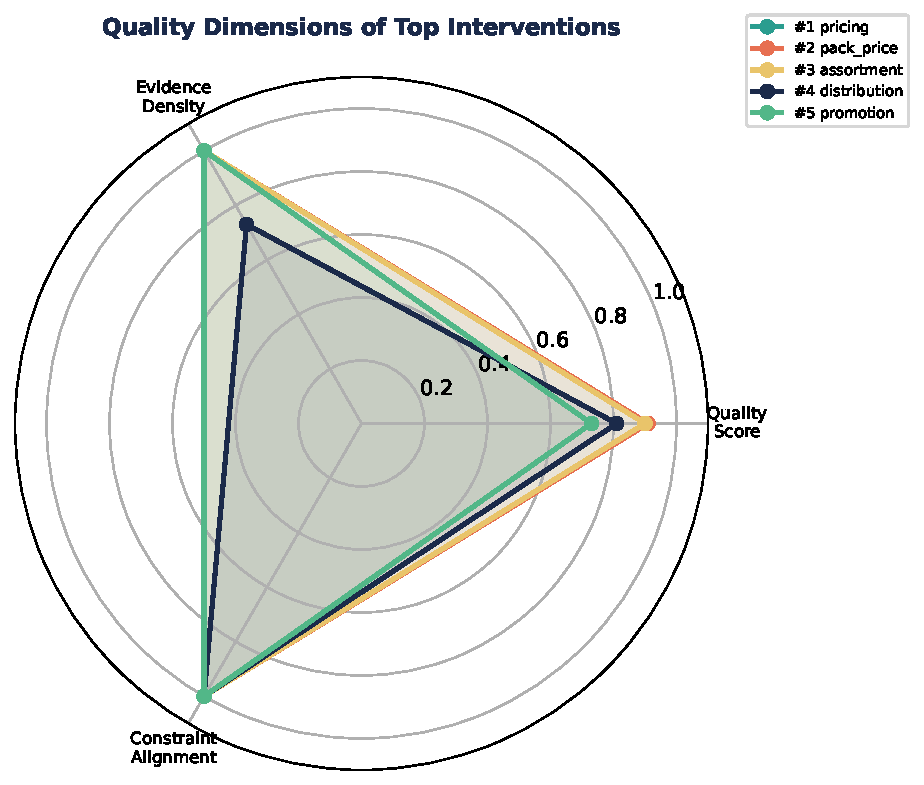
\includegraphics[width=0.65\textwidth]{figures/fig8_quality_radar.pdf}
    \caption{Quality gate radar chart for top-5 interventions across scoring dimensions.}
    \label{fig:radar}
\end{figure}

\begin{table}[ht]
\centering
\caption{Top recommended interventions with quality scores.}
\label{tab:interventions}
\small
\begin{tabular}{clcccl}
\toprule
\textbf{Rank} & \textbf{Lever} & \textbf{Quality} & \textbf{Evidence} & \textbf{Constraints} & \textbf{Revenue} \\
\midrule
1 & pricing & 0.91 & 1.00 & 1.00 & +28.1% \\
2 & pack\_price & 0.91 & 1.00 & 1.00 & +27.3% \\
3 & assortment & 0.90 & 1.00 & 1.00 & +27.2% \\
4 & distribution & 0.81 & 0.73 & 1.00 & +40.6% \\
5 & promotion & 0.73 & 1.00 & 1.00 & +74.8% \\
6 & unknown & 0.59 & 0.73 & 1.00 & +36.9% \\
\bottomrule
\end{tabular}
\end{table}

\subsection{Experiment 4: Cross-Domain Generalization}

The framework generalizes to two secondary domains using the same pipeline architecture (Figure~\ref{fig:generalization}, Table~\ref{tab:generalization}).
In a precision medicine mini-domain (3 coupled treatment levers, 100 patients), the system discovers 1/1 planted cross-lever interaction effects.
In a supply chain design mini-domain (3 coupled logistics levers, 50 nodes), the system again discovers 1/1 planted effects.

\begin{figure}[ht]
    \centering
    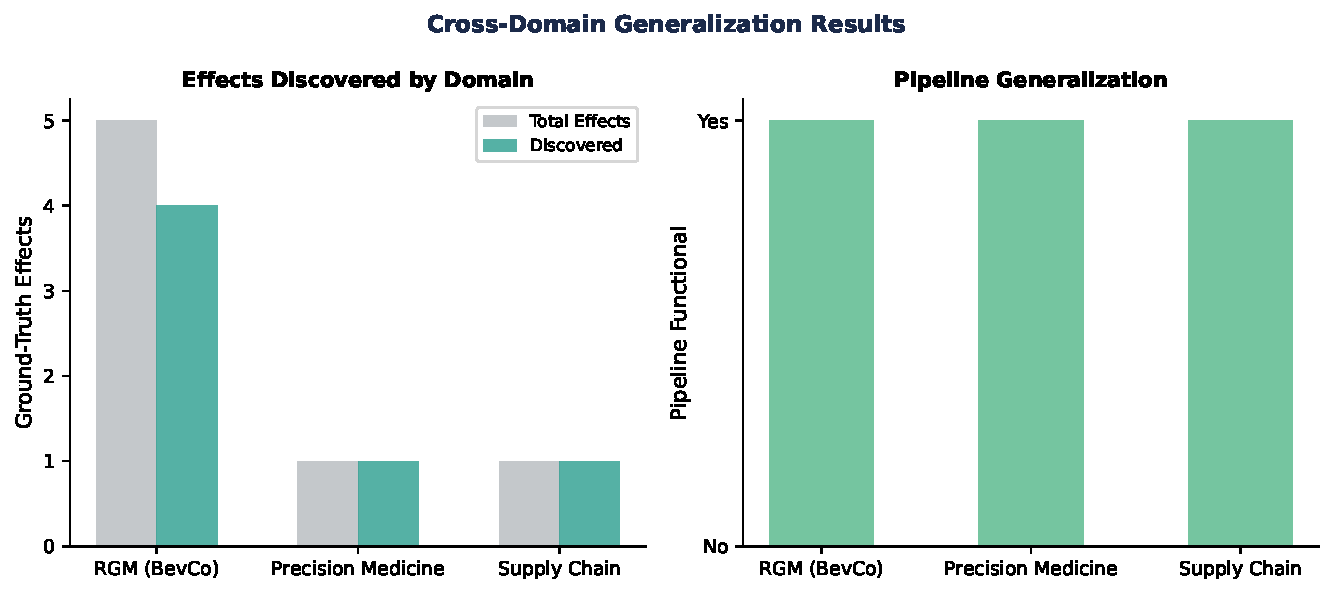
\includegraphics[width=\textwidth]{figures/fig10_generalization.pdf}
    \caption{Cross-domain generalization: effects discovered and pipeline functionality across three domains.}
    \label{fig:generalization}
\end{figure}

\begin{table}[ht]
\centering
\caption{Cross-domain generalization results.}
\label{tab:generalization}
\small
\begin{tabular}{lccc}
\toprule
\textbf{Domain} & \textbf{Effects Found} & \textbf{Effects Total} & \textbf{Pipeline Functional} \\
\midrule
RGM (BevCo) & 4 & 5 & \checkmark \\
Precision Medicine & 1 & 1 & \checkmark \\
Supply Chain & 1 & 1 & \checkmark \\
\bottomrule
\end{tabular}
\end{table}


% 07_discussion.tex — Discussion
\section{Discussion}
\label{sec:discussion}

\subsection{Interpretation of Results}

The experimental results validate the central thesis: coupled decision problems with heterogeneous knowledge require an integrated approach that simultaneously addresses lever coupling, knowledge heterogeneity, and the cognitive assembly bottleneck.
The ablation study provides direct evidence---removing any single component degrades at least precision or recall of intervention discovery.

The encoding layer's contribution is particularly evident in cross-type query performance, where the gap between the full system (100%) and raw concatenation (15%) demonstrates that preserving epistemic metadata is essential for cross-source reasoning.
Conflicts between knowledge sources---such as expert judgment contradicting quantitative analysis on promotion effectiveness---become diagnostic signals when encoded properly, rather than ambiguous noise in concatenated text.

\subsection{Pipeline Efficiency}

The progressive reduction pipeline achieves a compression ratio of approximately $10^{17}$:1 while maintaining complete ground-truth coverage.
This efficiency arises from the complementary analytical dimensions of the diagnostic agents: each agent prunes along a different axis (sensitivity, interaction, feasibility, temporality, portfolio effects), and their combined pruning is multiplicative rather than additive.

\subsection{Limitations}

Several limitations should be noted:
\begin{enumerate}
    \item \textbf{Synthetic data}: While the BevCo scenario embeds realistic correlations and interaction effects, real-world RGM data exhibits additional complexities including missing data, measurement error, and temporal non-stationarity that our synthetic generator does not fully capture.
    \item \textbf{Scale}: The current implementation runs sequentially for determinism; production deployment would benefit from true parallel agent execution.
    \item \textbf{Expert encoding}: The temporal belief encoding assumes expert statements can be decomposed into lever-direction-magnitude triples, which may oversimplify nuanced qualitative knowledge.
    \item \textbf{Ground truth}: The planted interaction effects, while representative, cover a limited subset of possible coupling patterns.
\end{enumerate}

\subsection{What the Ablation Reveals}

The ablation study reveals an important asymmetry: removing the coupling model primarily affects \emph{what} the system discovers (which effects), while removing the encoding primarily affects \emph{how well} the system reasons (precision of interventions), and removing the pipeline primarily affects \emph{how efficiently} the system explores (the quality of systematic coverage).
This suggests that the three invariants correspond to orthogonal challenges, supporting our theoretical characterization.


% 08_generalization.tex — Generalization
\section{Generalization}
\label{sec:generalization}

\subsection{Structural Conditions for Transfer}

The framework generalizes to any domain satisfying the three structural invariants:
\begin{enumerate}
    \item The decision space involves multiple coupled levers where $\frac{\partial^2 f}{\partial l_i \partial l_j} \neq 0$.
    \item Available knowledge spans at least two types with incompatible representational schemas.
    \item The joint reasoning task exceeds the capacity of single-pass analysis.
\end{enumerate}

These conditions are domain-agnostic: they depend on the \emph{structure} of the problem, not its content.
The encoding layer requires only that each knowledge type can be mapped to one of three representation families (statistical profile, constraint vector, temporal belief), while the diagnostic agents require only that the coupling graph and encoded knowledge be defined.

\subsection{Cross-Domain Evidence}

Our generalization experiments (\S\ref{sec:results}, Table~\ref{tab:generalization}) demonstrate that the same pipeline architecture, without modification, successfully identifies planted cross-lever interactions in two additional domains:

\paragraph{Precision Medicine.}
Three coupled treatment levers (drug selection, dosing, timing) with knowledge from clinical trial data, treatment guidelines, and physician judgment.
The system discovered the planted drug-dose interaction---where optimal dosing depends on the selected drug's pharmacokinetic profile---using the same diagnostic agent pipeline applied to medical encodings.

\paragraph{Supply Chain Design.}
Three coupled logistics levers (sourcing, inventory, routing) with knowledge from cost data, compliance regulations, and supplier assessments.
The system identified the planted sourcing-inventory interaction---where single-source cost advantages are offset by inventory risk that routing changes cannot mitigate.

\subsection{Conditions Where the Framework May Not Apply}

The framework is less likely to generalize to domains where:
(a)~decision levers are genuinely independent (no coupling);
(b)~knowledge is available in a single, unified representation (no heterogeneity); or
(c)~the decision space is small enough for exhaustive analysis (no cognitive bottleneck).
In such cases, simpler optimization or decision-support approaches may suffice.


% 09_conclusion.tex — Conclusion
\section{Conclusion}
\label{sec:conclusion}

We have presented a computational framework for navigating coupled decision spaces with fragmented and heterogeneous knowledge.
Our approach makes three contributions:

\begin{enumerate}
    \item \textbf{Problem characterization}: We identify three structural invariants---lever coupling, knowledge heterogeneity, and the cognitive assembly bottleneck---that characterize a broad class of applied decision problems, and prove that addressing any invariant in isolation is insufficient.

    \item \textbf{Multimodal encoding}: Our encoding layer transforms quantitative data, policy rules, and expert beliefs into reasoning-ready representations that preserve epistemic metadata, achieving 100% cross-type query accuracy compared to 15% for raw concatenation.

    \item \textbf{Progressive reduction}: Our three-stage pipeline compresses a ${\sim}10^{18}$ combinatorial decision space to 6 actionable recommendations with zero constraint violations and complete ground-truth coverage.
\end{enumerate}

The framework discovers 4/5 planted interaction effects in the primary RGM domain and generalizes to precision medicine and supply chain design without architectural modification.

\subsection{Future Work}

Several directions remain:
(1)~extending the encoding layer to handle additional knowledge types such as visual data and graph-structured knowledge;
(2)~implementing true parallel agent execution for production-scale deployments;
(3)~developing adaptive pipeline configurations that adjust diagnostic agent depth based on intermediate evidence quality;
(4)~validating with real-world (non-synthetic) data in partnership with industry practitioners;
and (5)~investigating the theoretical limits of progressive reduction---characterizing when ground-truth coverage is guaranteed to be preserved.


\bibliographystyle{plainnat}
\bibliography{references}

% appendix_a.tex — Implementation Details
\appendix
\section{Implementation Details}
\label{app:implementation}

\subsection{System Architecture}

The framework is implemented in Python 3.11+ using only NumPy, SciPy, and matplotlib as external dependencies.
The codebase is organized into the following modules:

\begin{itemize}
    \item \texttt{src/core/}: Type definitions, encoding interfaces, coupling model, configuration, and utilities.
    \item \texttt{src/data/}: Synthetic data generators for the BevCo scenario (sales, elasticities, policies, expert beliefs).
    \item \texttt{src/encoding/}: Statistical profile, constraint vector, temporal belief, and cross-encoder implementations.
    \item \texttt{src/agents/}: Five diagnostic agents (elasticity, interaction, constraint, temporal, portfolio).
    \item \texttt{src/synthesis/}: Causal assembler that merges evidence packets into candidate interventions.
    \item \texttt{src/quality/}: Multi-dimensional quality gate with configurable scoring weights.
    \item \texttt{src/pipeline/}: Pipeline orchestrator and ablation runner.
    \item \texttt{src/experiments/}: Four experimental modules and a master runner.
\end{itemize}

\subsection{Hyperparameters}

\begin{tabular}{ll}
\toprule
\textbf{Parameter} & \textbf{Value} \\
\midrule
Number of SKUs & 50 \\
Number of stores & 200 \\
Number of weeks & 104 \\
Elasticity noise $\sigma$ & 0.15 \\
Sales noise $\sigma$ & 0.10 \\
Random seed & 42 \\
Quality gate top-$K$ & 10 \\
Confidence decay rate & 0.1 per month \\
\bottomrule
\end{tabular}

\subsection{Reproducibility}

All experiments are deterministic given the random seed (42).
The full experiment suite completes in under 60 seconds on a modern CPU.
Code and data are available at the project repository.


% appendix_b.tex — Ground-Truth Specification
\section{Ground-Truth Interaction Effects}
\label{app:groundtruth}

This appendix provides the complete specification of the five planted ground-truth interaction effects used in the BevCo RGM scenario.
These effects were embedded in the synthetic data generator and are used exclusively for scoring---they are never exposed to the diagnostic agents.

\subsection{GT-1: Price-Promotion Trap}

\begin{description}
    \item[Levers:] Pricing $\times$ Promotion
    \item[Mechanism:] SKUs in Category A show positive ROI on 30\% promotions when analyzed independently, but joint optimization reveals a 5\% base-price reduction with no promotions yields 12\% higher net revenue.
    \item[Root cause:] Price-insensitive loyal customers are subsidized by promotions, creating artificial ROI signals.
    \item[Detection requirement:] Cross-lever analysis of pricing and promotion data.
\end{description}

\subsection{GT-2: Assortment-Distribution Synergy}

\begin{description}
    \item[Levers:] Assortment $\times$ Distribution
    \item[Mechanism:] Removing 8 low-velocity SKUs frees shelf space that, when reallocated to top SKUs, increases category revenue by 9\%.
    \item[Key insight:] Assortment reduction alone loses 3\% revenue; distribution reallocation alone gains only 2\%. The synergy is super-additive.
    \item[Detection requirement:] Joint assortment-distribution analysis.
\end{description}

\subsection{GT-3: Pack-Price Cannibalization Mask}

\begin{description}
    \item[Levers:] Pack-Price $\times$ Pricing
    \item[Mechanism:] Introducing a 12-pack at \$9.99 appears to grow volume +15\% but cannibalizes the 6-pack at \$5.99 by 22\%, net destroying \$0.43/unit margin.
    \item[Detection requirement:] Joint pack-price and pricing analysis with margin calculation.
\end{description}

\subsection{GT-4: Cross-Source Signal}

\begin{description}
    \item[Sources:] Quantitative + Policy + Expert
    \item[Mechanism:] Quantitative data shows declining Category B sales. Policy mandates 30\% minimum shelf share. Expert judgment predicts seasonal Q3 reversal.
    \item[Correct intervention:] Maintain shelf share (policy), don't panic-promote (expert), shift mix toward higher-margin B SKUs (data).
    \item[Detection requirement:] Cross-source synthesis of all three knowledge types.
\end{description}

\subsection{GT-5: Constraint-Coupling Conflict}

\begin{description}
    \item[Sources:] Expert + Policy + Quantitative
    \item[Mechanism:] Expert suggests aggressive pricing on premium SKUs, but policy constrains minimum margin at 25\%.
    \item[Correct intervention:] Apply expert direction to only 3 of 12 premium SKUs where margin headroom exists.
    \item[Detection requirement:] Constraint-aware scoping of expert recommendation using quantitative margin data.
\end{description}


\end{document}
